\setcounter{step}{0}
%------------------------------------------
% information doc
\subsection{Donuty}
\PrepTime{30}
\CookingTime{10}
\CookingTempe{180}
\TypeCooking{Vyprážanie}
\NbPerson{4}
\Image{0 0 275 275}{images/donuty} %style 2
%------------------------------------------

\begin{ingredient}
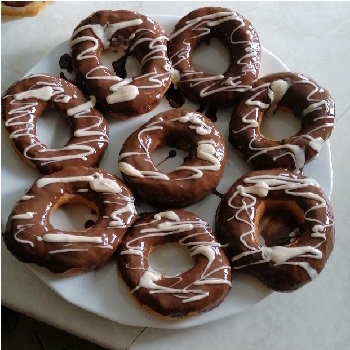
\includegraphics[height=5.5cm]{images/donuty}
\def\portions{4}%
\textbf{{\normalsize Ingrediencie (\portions porcie):}}
%\vspace{0.5cm}
\begin{main}
	\item štvrť maslo (65g)
	\item 2 PL kryštálový cukor
	\item vanilková aróma
	\item 1 vajce
	\item 2 hrnčeky polohrubá múka
\end{main}
\begin{subingredient}{Kvások}
	\item 1 hrnček teplé mlieko
	\item polovica droždie
	\item trošku cukor
\end{subingredient}
\end{ingredient}
\begin{recipe}
\textbf{{\normalsize Príprava:}}
\begin{enumerate}


\item{Vyrobíme kvások a necháme 30 minút kysnúť}
\item{Zmiešame zvyšné ingrediencie s kváskom}
\item{Vyvaľkáme na 1,5cm a povykrajujeme donuty}	
\item{Rozohrejeme olej s ČL masla}
\item{Opražíme tak 10s z jednej a 10s z druhej strany}
\item{Podľa ľubovôle poleva z čokolády}

\end{enumerate}
\end{recipe}

\begin{notes}

\end{notes}
\clearpage	